\documentclass{article}

\usepackage[T1]{fontenc}
\usepackage[utf8]{inputenc}
\usepackage{times}

\usepackage[font=small,labelfont=bf,tableposition=top]{caption}
\usepackage{graphicx}
\usepackage{natbib} 

\usepackage{amsmath}
\usepackage{amsfonts}
\usepackage{amssymb}
\usepackage{color, soul}
\usepackage{hyperref}
\usepackage{algorithmicx}
\usepackage{algpseudocode}
\usepackage{subfigure}
\usepackage{stmaryrd}
\usepackage{mathrsfs}
\usepackage[inline]{enumitem}
\usepackage{hyperref}
\newcommand{\comment}[1]{}
\usepackage{bbm}
\hypersetup{
    colorlinks=true,
    linkcolor=blue,
    citecolor=blue,
    filecolor=cyan,      
    urlcolor=cyan,
}

\usepackage{empheq}
\definecolor{paleblue}{rgb}{.8, .8, 1} 
\newcommand*\eqnbox[1]{%
    \colorbox{paleblue}{\hspace{1em}#1\hspace{1em}}}
\newcommand{\hlpaleblue}[1]{{\sethlcolor{paleblue}\hl{#1}}}

\renewcommand{\vec}[1]{\boldsymbol{{#1}}} 
\DeclareMathOperator\atanh{atanh}

\newcommand{\laplacian}{\nabla^2}
\newcommand{\divergence}{\nabla \cdot}
\newcommand{\grad}{\nabla}
\newcommand{\Grad}{\nabla}

\newtheorem{theorem}{Theorem}
 \newtheorem{acknowledgement}[theorem]{Acknowledgement}
 \newtheorem{algorithm}[theorem]{Algorithm}
 \newtheorem{axiom}[theorem]{Axiom}
 \newtheorem{case}[theorem]{Case}
 \newtheorem{claim}[theorem]{Claim}
 \newtheorem{conclusion}[theorem]{Conclusion}
 \newtheorem{condition}[theorem]{Condition}
 \newtheorem{conjecture}[theorem]{Conjecture}
 \newtheorem{corollary}[theorem]{Corollary}
 \newtheorem{criterion}[theorem]{Criterion}
 \newtheorem{definition}[theorem]{Definition}
 \newtheorem{example}[theorem]{Example}
 \newtheorem{exercise}[theorem]{Exercise}
 \newtheorem{lemma}[theorem]{Lemma}
 \newtheorem{notation}[theorem]{Notation}
 \newtheorem{problem}[theorem]{Problem}
 \newtheorem{proposition}[theorem]{Proposition}
 \newtheorem{remark}[theorem]{Remark}
 \newtheorem{solution}[theorem]{Solution}
 \newtheorem{summary}[theorem]{Summary}
 \newenvironment{proof}[1][Proof]{\textbf{#1.} }{\ \rule{0.5em}{0.5em}}

\newcommand{\Norder} {N}
\newcommand{\order}{\mathcal{O}}
\newcommand{\Npoints} {N_p}
\newcommand{\Nfaces} {N_{f}}
\newcommand{\Nelements} {N_e}

\newcommand{\eps}{\varepsilon}
\newcommand{\Dweak}{\wt{D}}
\newcommand{\diff}[2] {\frac{\partial #1}{\partial #2}}
\newcommand{\dxx}[2] {\frac{\partial^2 #1}{\partial {#2}^2}}
\newcommand{\difft}[2] {\frac{d #1}{d #2}}
\newcommand{\dxxt}[2] {\frac{d^2 #1}{d {#2}^2}}
\newcommand{\lagrange}[1] {\frac{d #1}{dt}}
\newcommand{\lebesgue}{\parallel I \parallel}
\newcommand{\polysp}{\mathcal{P}_N}

\newcommand{\inte}{\int_{\mbox{\footnotesize ${\Omega_e}$}}}
\newcommand{\intb}{\int_{\mbox{\footnotesize ${\Gamma_e}$}}}
\newcommand{\intce}{\int_{\mbox{\footnotesize ${\widehat{\Omega}_e}$}}}
\newcommand{\intcb}{\int_{\mbox{\footnotesize ${\widehat{\Gamma}_e}$}}}
\newcommand{\intg}{\int_{\mbox{\footnotesize ${\Omega}$}}}
\newcommand{\intgb}{\int_{\mbox{\footnotesize ${\Gamma}$}}}
\newcommand{\intv}{\int_{\mbox{\footnotesize ${\sigma}$}}}
\newcommand{\sumv}{\sum_{K=1}^{N_{\mathrm{lev}}}}
\newcommand{\sumk}{\sum_{L=1}^{K}}
\newcommand{\sumN}{\sum_{i=1}^{N+1}}
\newcommand{\half}{\frac{1}{2}}
\newcommand{\inti}{\int_{\mbox{\footnotesize\sf I}}}
\newcommand{\intbd}{\oint_{\mbox{\footnotesize ${\delta}$\sf D}}}
\newcommand{\intbi}{\oint_{\mbox{\footnotesize ${\delta}$\sf I}}}
\newcommand{\ldnorm}[1]{\left\| #1 \right\|_{\mbox{\footnotesize \sf D}} }
\newcommand{\lonorm}[1]{\left\| #1 \right\|_{\Omega}}
\newcommand{\spc}[1]{\mbox{\sf #1}}
\newcommand{\ope}[1]{{\cal #1}}
\newcommand{\mt}[1]{{\rm #1}}
\newcommand{\dis}{\displaystyle}
\newcommand{\ve}{\varepsilon}
\newcommand{\ov}{\overline}
\newcommand{\wt}{\widetilde}
\newcommand{\wh}{\widehat}
\newcommand{\Dhat}{\widehat{D}}
\newcommand{\be}{\begin{equation}}
\newcommand{\ee}{\end{equation}}
\newcommand{\bea}{\begin{eqnarray*}}
\newcommand{\eea}{\end{eqnarray*}}
\newcommand{\Jace}{J^{(e)}}
\newcommand{\Jacl}{J^{(l)}}
\def\bepsilon{\mbox{\boldmath $\epsilon $}}
\def\bpsi{\mbox{\boldmath $\psi $}}
\def\bphi{\mbox{\boldmath $\phi $}}
\def\bmu{\mbox{\boldmath $\mu $}}
\def\Et{ \tilde{E} }
\def\Ht{ \tilde{H} }
\def\sdot{ \dot{\sigma} }

\newcommand{\fstar}{f^{(*)}}

\DeclareMathOperator{\Span}{span}
\DeclareMathOperator{\Dim}{dim}

\newcommand{\polyquad}{\mathcal{Q}_{N}}
\newcommand{\polyP}{\mathcal{P}_{N}}
\newcommand{\polyPnpm}{\mathcal{P}_{(N+M)}}
\newcommand{\polyPd}{\mathcal{P}_{d}}
\newcommand{\polyPnm}{\mathcal{P}_{N,M}}
\newcommand{\polyPn}{\mathcal{P}_{N,0}}
\newcommand{\transpose}{^{\mathcal{T}}}

\newcommand{\vecQ}{\vec{Q}}
\newcommand{\vecQe}{\vec{Q}^{(e)}}
\newcommand{\vecFe}{\vec{\mathcal{F}}^{(e)}}
\newcommand{\statevec}{\vec{Y}}
\newcommand{\statevecN}{\vec{Y}_N^{(e)}}
\newcommand{\statestage}{\vec{\mathcal{Y}}}
\newcommand{\Ftensor}{\vec{F}(\qvector)}
\newcommand{\FtensorN}{\vec{F}\left( \qvectorN \right)}
\newcommand{\FtensorStar}{\vec{F}\left( \qvector_N^{(e,k)} \right)}
\newcommand{\Svector}{S(\qvector)}
\newcommand{\SvectorN}{S \left( \qvectorN \right)}
\newcommand{\qref}{\vec{q}_0}
\newcommand{\qvectorb}{\vec{q}_b}
\newcommand{\qtt}{\vec{q}_{tt}}
\newcommand{\qhat}{\widehat{\vec{q}}}
\newcommand{\qhatb}{\widehat{\vec{q}}_b}
\newcommand{\qelem}{q^{(e)}}
\newcommand{\rhoref}{\rho_0}
\newcommand{\piref}{\pi_0}
\newcommand{\Thetaref}{\Theta_0}
\newcommand{\Gref}{G_0}
\newcommand{\Tref}{T_0}
\newcommand{\thetaref}{\theta_0}
\newcommand{\Pref}{{P}_0}
\newcommand{\Eref}{{E}_0}
\newcommand{\Href}{{h}_0}
\newcommand{\rhohat}{\widehat{\rho}}
\newcommand{\pihat}{\widehat{\pi}}
\newcommand{\Phat}{\widehat{P}}
\newcommand{\uvechat}{\widehat{{\mbox{\boldmath$u$\unboldmath}}}}
\newcommand{\uhathat}{\widehat{\widehat{{\mbox{\boldmath$u$\unboldmath}}}}}
\newcommand{\Uhat}{\widehat{{\mbox{\boldmath$U$\unboldmath}}}}
\newcommand{\Uhathat}{\widehat{\widehat{{\mbox{\boldmath$U$\unboldmath}}}}}
\newcommand{\thetahat}{\widehat{\theta}}
\newcommand{\Thetahat}{\widehat{\Theta}}
\newcommand{\Ehat}{\widehat{E}}
\newcommand{\uhat}{\widehat{u}}
\newcommand{\vhat}{\widehat{v}}
\newcommand{\what}{\widehat{w}}
\newcommand{\pitt}{\pi_{tt}}
\newcommand{\rhott}{\rho_{tt}}
\newcommand{\Ett}{E_{tt}}
\newcommand{\Utt}{\vec{U}_{tt}}
\newcommand{\uvectt}{\vec{u}_{tt}}
\newcommand{\utt}{u_{tt}}
\newcommand{\vtt}{v_{tt}}
\newcommand{\wtt}{w_{tt}}
\newcommand{\Ptt}{P_{tt}}
\newcommand{\vecPtt}{\vec{P}_{tt}}
\newcommand{\Thetatt}{\Theta_{tt}}
\newcommand{\thetatt}{\theta_{tt}}
%Projector Matrices
\newcommand{\projmatrix}{\vec{\mathcal{P}}}
\newcommand{\qmatrix}{\vec{\mathcal{Q}}}
\newcommand{\pcmatrix}{\vec{\mathcal{P}}_C}
\newcommand{\Cmatrix}{\left(\vec{\mathcal{C}}^{(e,f)}\right)\transpose}
\newcommand{\Dmatrix}{\vec{D}^{(e)}}
\newcommand{\Dwmatrix}{\wt{\vec{D}}^{(e)}}
\newcommand{\Mmatrix}{M^{(e)}}
\newcommand{\Fmatrix}{\vec{F}^{(e,l)}}
\newcommand{\Gmatrix}{\mathcal{G}}
\newcommand{\Umatrix}{\mathcal{U}^{(e,f)}}
\newcommand{\amatrix}{\vec{\mathcal{A}}}
\newcommand{\rmatrix}{\vec{\mathcal{R}}}
%Vectors
\newcommand{\nvector}{\wh{\vec{n}}_{\Gamma}}
\newcommand{\nhat}{\wh{\vec{n}}}
\newcommand{\ivector}{\wh{\vec{i}}}
\newcommand{\jvector}{\wh{\vec{j}}}
\newcommand{\kvector}{\wh{\vec{k}}}
\newcommand{\rvector}{\wh{\vec{r}}}
\newcommand{\svector}{\wh{\vec{s}}}
\newcommand{\tvector}{\wh{\vec{t}}}
\newcommand{\vvector}{\wh{\vec{v}}}
\newcommand{\Qvector}{\vec{Q}}
%Vectors
\newcommand{\ur}{{u}^{(r)}}
\newcommand{\us}{{u}^{(s)}}
\newcommand{\ut}{{u}^{(t)}}
\newcommand{\urtt}{{u}_{tt}^{(r)}}
\newcommand{\ustt}{{u}_{tt}^{(s)}}
\newcommand{\uttt}{{u}_{tt}^{(t)}}
\newcommand{\urhat}{\widehat{u}^{(r)}}
\newcommand{\ushat}{\widehat{u}^{(s)}}
\newcommand{\uthat}{\widehat{u}^{(t)}}
%Other Operators

\newcommand{\Dskew}{\mathcal{D}}

\def\bepsilon{\mbox{\boldmath $\epsilon $}}
\def\bpsi{\mbox{\boldmath $\psi $}}
\def\bphi{\mbox{\boldmath $\phi $}}
\def\bmu{\mbox{\boldmath $\mu $}}
\def\Et{ \tilde{E} }
\def\Ht{ \tilde{H} }
\def\sdot{ \dot{\sigma} }
%\renewcommand{\thetable}{\Roman{table}}
%\renewcommand{\thefigure}{\arabic{figure}}

%\DeclareMathOperator{\Span}{span}
%\DeclareMathOperator{\Dim}{dim}

%Editing Commands
\newcommand{\here}{ \textcolor{red}{YOU ARE HERE}}
\newcommand{\red}[1]{ \textcolor{red}{#1}} 
\newcommand{\blue}[1]{ \textcolor{blue}{#1}}
\newcommand{\magenta}[1]{ \textcolor{magenta}{#1}}

%Time-Integration
\newcommand{\dt}{{\Delta t}}
\newcommand\ST{\rule[-0.75em]{0pt}{2em}}
\newcommand{\Sfunction}{\mathcal{S}}
\newcommand{\Lfunction}{\mathcal{L}}
\newcommand{\Nfunction}{\mathcal{N}}

%DG Operators
\newcommand{\average}[1]{ \left\{ #1 \right\} }
\newcommand{\jump}[1]{ \llbracket #1 \rrbracket }

%HDG Matrices
\newcommand{\CCmatrix}{\mathcal{C}^{(e,k)}}
\newcommand{\Jmatrix}{\mathcal{J}^{(e,k)}}
\newcommand{\DDmatrix}{\wt{D}^{(e)}}
\newcommand{\SSvector}{\mathcal{S}(q)}
\newcommand{\cghdg}{cg\underline{\hspace{0.15cm}}to\underline{\hspace{0.15cm}}hdg}
%\newcommand{\ul}{\underline{\hspace{0.15cm}}}
\newcommand{\RRmatrix}{\mathcal{R}}

%Clima specific variables
\newcommand{\etotal}{e^{\mathrm{tot}}}
\newcommand{\Etotal}{E^{\mathrm{tot}}}
\newcommand{\Fvector}{\vec{\mathcal{F}}}
\newcommand{\Hvector}{\vec{\mathcal{H}}}
\newcommand{\Pvector}{\vec{\mathcal{P}}}
\newcommand{\Fndiff}{\vec{\mathcal{F}}^{\mathrm{nondiff}}}
\newcommand{\Frad}{\vec{\mathcal{F}}^{\mathrm{rad}}}
\newcommand{\Ffall}{\vec{\mathcal{F}}^{\mathrm{fall}}}
\newcommand{\Fdiff}{\vec{\mathcal{F}}^{\mathrm{diff}}}
\newcommand{\Fnondiff}{\vec{\mathcal{F}}^{\mathrm{nondiff}}}
\newcommand{\Tvector}{\vec{\mathcal{T}}}
\newcommand{\Source}{\vec{\mathcal{S}}}

%DG specific variables
\newcommand{\Yvector}{\vec{\mathcal{Y}}}
%\newcommand{\Fvector}{\vec{\mathcal{F}}}. % already defined!
%\newcommand{\Svector}{\vec{\mathcal{H}}}
%\newcommand{\Hvector}{\vec{\mathcal{H}}}
\newcommand{\Gvector}{\vec{\mathcal{G}}}
\newcommand{\Dvector}{\vec{\mathcal{D}}}


\newcommand{\fxg}[1]{\textcolor{cyan}{FXG: #1}}



\title{CLIMA Atmosphere Model Benchmarks}
\author{ }

\begin{document}

\maketitle
\tableofcontents

\section{Held-Suarez (1994) Dry GCM Benchmark}

Charlie is trying to see if the benchmarks can be split off from the design docs / mathematical formulation. There are still unresolved references.

\section{Held-Suarez (1994) Dry GCM Benchmark}

\citet{Held94} describe a simple and widely used setup for testing dry dynamical cores of GCMs. This setup is usually used to focus on statistically steady states (reached after about 100--400~days of spinup) but also lends itself to the study of the time-dependent evolution of Rossby waves and baroclinic instability. In this benchmark calculation, vertical SGS fluxes are usually set to zero; however, horizontal diffusion (or hyperdiffusion) is needed to damp the enstrophy cascade. 

\subsubsection{Initial Condition}

The initial condition for the Held-Suarez benchmark is an isothermal atmosphere at rest, with $T(t=0) = 300~\mathrm{K}$. Hydrostatically balanced initial density and pressure fields are calculated from the initial temperature according to section~\ref{s:initial_conditions}, and some small random perturbations are added to the density field to break the symmetry of the initial state and allow 3D baroclinic waves to develop. Baroclinic waves develop within a few simulated days in this benchmark calculation, and they begin to equilibrate after around 20--30~days. 

\subsubsection{Boundary Conditions}

The lower boundary condition is free-slip and thermally insulating, with no evaporation. That is, \emph{all} diffusive fluxes at the lower boundary (see section~\ref{s:bottom_bc}) are taken to be zero (if they are not already taken to be zero throughout the atmosphere, which is common in the Held-Suarez benchmark). With the vanishing surface fluxes, there is no need to specify a surface temperature.

\subsubsection{Sources}

\paragraph{Momentum} Bottom drag in this benchmark calculation is modeled as a momentum sink in the lower part of the atmosphere, which is a function of velocity $\vec{u}$ and pressure $p$. The momentum sink takes the form of linear Rayleigh drag
\begin{equation}
    \vec{F}_u = -k_v(\sigma) \vec{u},
\end{equation}
where the drag coefficient decays away from the surface:
\begin{equation}
    k_v(\sigma) = k_f \max \left( 0, \frac{\sigma - \sigma_b}{1-\sigma_b} \right).
\end{equation}
Here,
\[
\sigma = \frac{p}{p_{\mathrm{MSLP}}}
\]
is a normalized pressure. (Usually, $\sigma$ is taken to be normalized by the temporally and spatially varying surface pressure $p_s$. But we can simplify this to a constant pressure.) \hl{[It would be good at some point to change this to the actual surface pressure, but this is not important now.]} The two parameters are
\begin{itemize}
    \item $\sigma_b = 0.7$: vertical extent of drag layer
    \item $k_f = 1~\mathrm{day^{-1}}$: drag coefficient at the surface
\end{itemize}.

\hl{Note that the momentum source appears in the momentum and energy equations. In hydrostatic models, the Rayleigh drag only acts on the horizontal velocity components and is zero in the vertical. Would that be easy to implement for us? Otherwise, also damping vertical velocities is ok for now, but it may need to strongly distorted upwelling and subsidence.}

\paragraph{Heating/cooling}

Radiative heating/cooling is represented by linear relaxation of temperatures toward a radiative-equilibrium state with temperature \hl{[Note that here $p/p_{\mathrm{MSLP}}$ should be this, with a constant pressure for normalization. So generally, this is not equal to $\sigma$ above; it is only with the simplified $\sigma$ above.]}
\begin{multline}
    T_{\mathrm{eq}} = \max \\
    \left\{ T_{\mathrm{top}}, \left[ T_{\max} - (\Delta T)_y \sin^2 \phi - (\Delta \theta)_z \log\left(\frac{p}{p_{\mathrm{MSLP}}}\right) \cos^2 \phi \right]
    \left( \frac{p}{p_{\mathrm{MSLP}}} \right)^{\kappa} \right\}.
\end{multline}
Here, $\phi$ is latitude, $\kappa = R_d/c_{pd}$ is the adiabatic exponent, and the default values of the parameters are:
\begin{itemize}
    \item $T_{\mathrm{top}} = 200~\mathrm{K}$: temperature at model top
    \item $T_{\max} = 315~\mathrm{K}$: near-surface temperature at equator
    \item $(\Delta T)_y = 60~\mathrm{K}$: pole-equator temperature difference in radiative equilibrium
    \item $(\Delta \theta)_z = 10~\mathrm{K}$: static stability in background state.
\end{itemize}

Relaxation of temperatures toward the background state on a timescale $k_T^{-1}$ implies a source in the energy equation that is a function of latitude $\phi$, pressure $p$, and temperature $T$:
\begin{equation}
    Q =  - c_{vd} k_T(\phi, p) (T - T_{\mathrm{eq}}).
\end{equation} 
The relaxation coefficient $k_T$ is taken to vary with latitude and normalized pressure $\sigma$ as
\begin{equation}
k_T(\phi, p) = k_a + (k_s - k_a) \max\left(0, \frac{\sigma - \sigma_b}{1-\sigma_b}\right) \cos^4 \phi ,
\end{equation}
where 
\begin{itemize}
    \item $k_a = (40~\mathrm{day})^{-1}$: relaxation coefficient in interior atmosphere
    \item $k_s = (4~\mathrm{day})^{-1}$: relaxation coefficient  at equator near the surface.
\end{itemize}
The interior relaxation timescale $k_a^{-1}$ controls the timescale over which they flow equilibrates to a statistically steady state

\subsubsection{SGS Fluxes}

In global models with a stratified atmosphere, large-scale turbulence with Rossby waves usually dominates the kinetic energy of the flow. The large-scale flow is primarily rotational and horizontal. SGS dissipation primarily needs to absorb the cascade of enstrophy (vorticity variance) to small scales. This is usually accomplished by horizontal hyperdiffusion.

Hence, the SGS mixing needs to be strongly anisotropic, e.g., as outlined in section~\ref{s:anisotropic_SGS_mixing}.

\section{2D Rising Thermal Bubble (Robert 1993)}
\label{2dRTBtest}
This test is described \cite{robert1993}. It consists of a flow that is triggered by the thermal perturbation of a neutrally stratified atmosphere at initially uniform potential temperature $\theta_0 = 303$ K
and in hydrostatic equilibrium such that the pressure decreases with $z$ as:
\begin{equation}
\label{pressureDistrib}
p = p_{0}\left(1-\frac{g}{c_p{\theta_{0}}}z\right)^{c_p/R}.
\end{equation}
The domain $\Omega=[-5000,5000]\times[0,10000]\,\mathrm{m}^2$.
The perturbation is linear and defined as
\begin{equation}
 \Delta\theta = \left\{ \begin{array}{ll}
 \theta_c & \mathrm{if } r \leq a=50\,{\mathrm K}\\
 \theta_c e^{-(x - a)^2/\sigma^2} & \mathrm{if } r > a=50\,{\mathrm K}\\
\end{array} \right.
\label{eq:robertIni}
\end{equation}
where $r = \sqrt[]{(x-x_{c})^{2} + (z-z_{c})^{2}}$, $(x_c,z_c) = (500,260)\,\mathrm{m}$, $\sigma = 100$, and $\theta_c=0.5$ K.

\begin{figure}[htbp]
\includegraphics[width=\textwidth]{figures/RTB-Robert--smgo-5mX5m-1080s0000.png}
\caption{2D rising thermal bubble (Robert, 1993) stabilized via a constant coefficient Smagorinsky-Lilly SGS: Potential temperature, $\theta$, at $t=1080\,\mathrm{s}$. Grid resolution: $\Delta x = \Delta z = 5\,\mathrm{m}$.}
\label{fig:benchmarks/robert5msmago}
\end{figure}

\section{2D Density Current}
This test is described in \cite{strakaWilhelmson1993}. It consists of a flow that is triggered by the cold perturbation of a neutrally stratified atmosphere at initially uniform potential temperature $\theta_0 = 300$ K
and in hydrostatic equilibrium such that the pressure decreases with $z$ as:
\begin{equation}
\label{pressureDistrib2}
p = p_{0}\left(1-\frac{g}{c_p{\theta_{0}}}z\right)^{c_p/R}.
\end{equation}
The domain $\Omega=[-25600,25600]\times[0,6400]\,\mathrm{m}^2$.
The perturbation is linear and defined as
\begin{equation}
 \Delta\theta = \left\{ \begin{array}{ll}
 0 & \mathrm{if } r > 1\,{\mathrm K}\\
 0.5 \theta_c \left(1 + \cos(\pi r) \right) \leq 1\,{\mathrm K}\\
\end{array} \right.
\label{eq:robertIni2}
\end{equation}
where $r = \sqrt[]{(x-x_{c})^2/r_x^{2} + (z-z_{c})^{2}/r_z^2}$, $(x_c,z_c) = (0,4000)\,\mathrm{m}$, $(r_x, r_z) = (4000, 2000)\,\mathrm{m}$ and $\theta_c=-15$ K. The fully developed density current at $t=900\,\mathrm{s}$ simulated with a grid effective resolution of $25$ m in both spatial directions is shown in Figure \ref{fig:benchmarks/dc25msmago}.

\begin{figure}[htbp]
\includegraphics[width=1.2\textwidth]{figures/DC-smgo-25mx25m-900s0000.png}
\caption{2D density current stabilized via a constant coefficient Smagorinsky-Lilly SGS. Potential temperature, $\theta$, at $t=900\,\mathrm{s}$ (top) and at $t=1200\,\mathrm{s}$ (bottom). Grid resolution: $\Delta x = \Delta z = 25\,\mathrm{m}$.
}
\label{fig:benchmarks/dc25msmago}
\end{figure}


%%
\section{Rising Thermal Bubble in a Saturated Atmosphere}
\label{rtb3D}
The moist dynamics is tested by means of the saturated rising bubble test described in \cite{Pressel15a}. The initial conditions are setup as follows:

\begin{itemize}
\item Initialize dry atmosphere with uniform background $\theta_{ref} = 320$ K
\item Add thermal perturbation $\Delta \theta$ of radius $r=2$ km
\item Set a uniform total mixing ratio $q_t = 0.0192 \,\mathrm{kg/kg}$ and $q_l = q_i = 0.0\,\mathrm{kg/kg}$
\item Calculate the gas constants for moist air: 
\[\begin{array}{lcl}
R_{gas} &=& {\tt MoistThermodynamics.gas\_constant\_air(q_t, q_l, q_i)}\\
c_v     &=& {\tt MoistThermodynamics.cv\_m(q_t, q_l, q_i)}\\
c_p     &=& {\tt MoistThermodynamics.cp\_m(q_t, q_l, q_i)}\\
\end{array}
\]
\item  Compute $\theta$, $\rho$, and $T$ as if the background were dry:\\
    \[ \begin{array}{lcl}
  \theta &=& \theta_{ref} + \Delta\theta\\
 \pi & =& 1 - gz/(c_p\theta)\\
 \rho & = & p_0/(R_{gas}\theta)\pi^{c_v/R_{gas}}\\
 T   & = &\pi \theta
\end{array}\]

\item Add the contribution of moisture to the internal energy and recalculate $T$ and $P$, and obtain $e^{\rm tot}$ using the following {\tt MoistThermodynamics} functions:
\[\begin{array}{lcl}
I &=& {\tt MoistThermodynamics.internal\_energy(T + T_0, q_t, q_l, q_i)}\\
T &=& {\tt MoistThermodynamics.air\_temperature(I, q_t, q_l, q_i)}\\
P &=& {\tt MoistThermodynamics.air\_pressure(T - T_{ref} , \rho, q_t, q_l, q_i)}\\
e^{\rm tot} &=& {\tt MoistThermodynamics.total\_energy(0.5\|{\bf u} \|^2, gz, T, q_t)}
\end{array}\]
\end{itemize}

%%
\section{Dynamics and Chemistry of Marine Stratocumulus: DYCOMS RF01}

\subsubsection{Initial Condition}

\cite{Stevens05a} provide the following initial distributions of liquid water potential temperature,
\begin{equation}\label{eq:dycoms1}
\theta_l(z) = 
    \begin{cases}
    289.0\;\mathrm{K} & z\leq z_i,\\
    297.5 + (z - z_i)^{1/3}\;\mathrm{K}& z > z_i,
    \end{cases}
\end{equation}
and total specific humidity, 
\begin{equation}\label{eq:dycoms2}
q_t(z) = 
    \begin{cases}
    q_{t,0} & z\leq z_i,\\
    1.5\;\mathrm{g/kg} & z > z_i.
    \end{cases}
\end{equation}
Here, $z_i$ is the initial cloud top set to $z_i=840\,\mathrm{m}$. \cite{Stevens05a} state that ``modeling groups were also asked to standardize their thermodynamic calculations'' so that the initial state corresponds to a cloud layer between 600 and 800~m with liquid water specific humidity
\begin{equation}\label{eq:dycoms3}
q_l(z) = 
    \begin{cases}
    0 & z\leq 600~\mathrm{m},\\
    0.45\frac{{}z - 600~\mathrm{m}}{z_i - 600~\mathrm{m}}\;\mathrm{\frac{g}{kg}}   & 600~\mathrm{m} < z \leq z_i,\\
    0 & z > z_i.\\
    \end{cases}
\end{equation}
With our thermodynamics and standard thermodynamical constants, we obtain such a cloud layer if we choose the initial total specific humidity in the mixed layer to be $q_{t,0} = 8.1\;\mathrm{g/kg}$, which is slightly lower than the DYCOMS default value of $9\;\mathrm{g/kg}$. (An alternative to modifying the initial $q_{t,0}$ would be to adjust, e.g., the latent heat of vaporization or the vapor pressure at the triple point to obtain the desired cloud layer with $q_{t,0} = 9\;\mathrm{g/kg}$.)

To specify the thermodynamic state completely, we additionally need to specify an initial density. We do so by first specifying an initial pressure
\[
p_0(z) = p_{s} \exp(-z/H), \qquad H = \frac{R_m T_{BL}}{g},
\]
where $R_m = R_m(q_t, q_l)$ is the gas constant for moist air, $T_{BL} = 285.0~\mathrm{K}$ is an average boundary-layer temperature, and $p_s = 1.0178\times 10^{5}~\mathrm{Pa}$ is the surface pressure, with surface density $\rho_s = 1.22~\mathrm{kg/m^3}$ and surface temperature $T_s = p_s/(\rho_s R_{m,s})$. Consistent with the Boussinesq or anelastic approximation used in most DYCOMS simulations, we calculate thermodynamic quantities with this reference pressure $p_0(z)$. We use the linearized expression for the liquid-water potential temperature,
\begin{equation}
    \label{eq:betts1973}
    \theta_l = \theta \left(1 - \frac{L_{v,0} q_l}{c_{pm} T} \right) = \theta - \frac{L_{v,0} q_l}{c_{pm} \Pi_0},
\end{equation}
where $\theta = T/\Pi_0$, and 
\[
\Pi_0 = \left( \frac{p_0(z)}{p_{s}} \right)^{R_d/c_{pd}}
\]
is evaluated with the pressure profile $p_0(z)$. This can be solved for temperature as a function of height $z$,
\[
T = \Pi_0 \theta_l + \frac{L_{v,0} q_l}{c_{pm} \Pi_0},
\]
given $\theta_l(z)$, $q_l(z)$, and $\Pi(z)$. Density is then obtained from the ideal gas law as
\[
\rho(z) \approx \frac{p_0(z)}{R_m T(z)},
\]
thus completely specifying the initial state. 

The initial state of all the quantities described above are plotted in Figure \ref{dycomsInitFig}
\begin{figure}
    \centering
	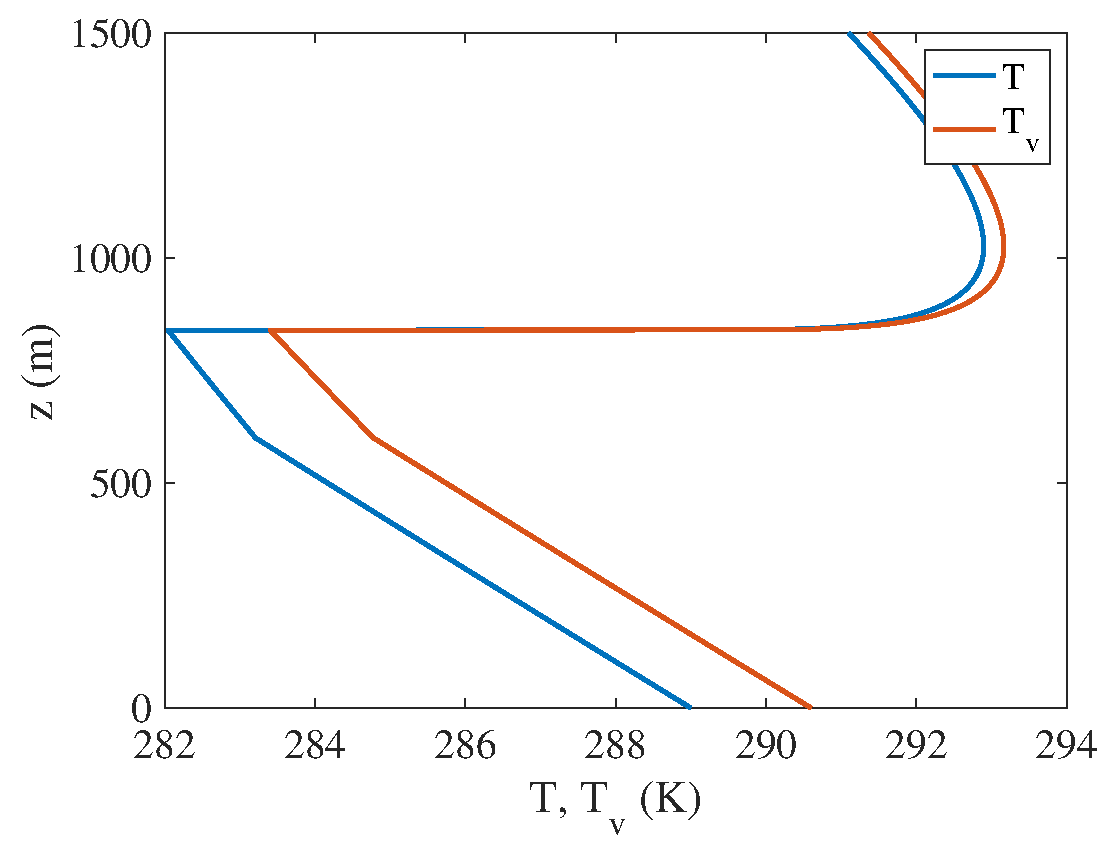
\includegraphics[width=0.49\textwidth]{./figures/dy_tempe.eps}
	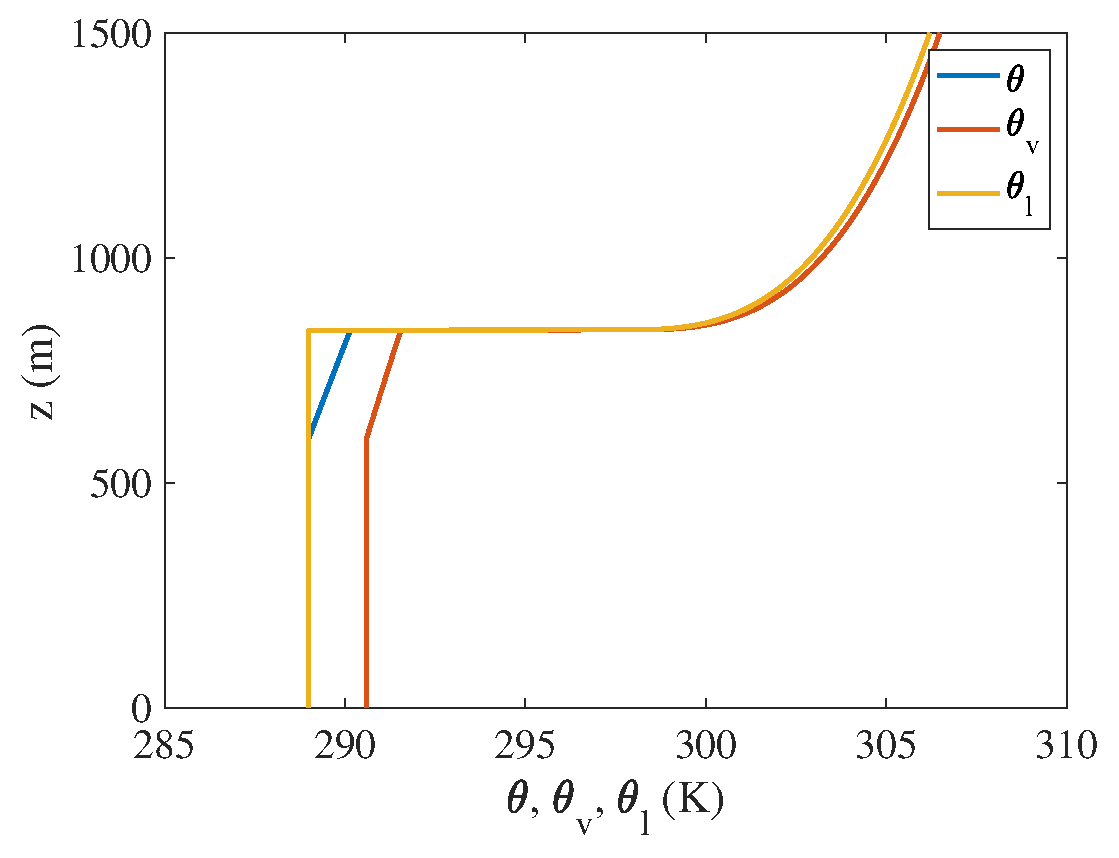
\includegraphics[width=0.49\textwidth]{./figures/dy_pot_temp.eps}
	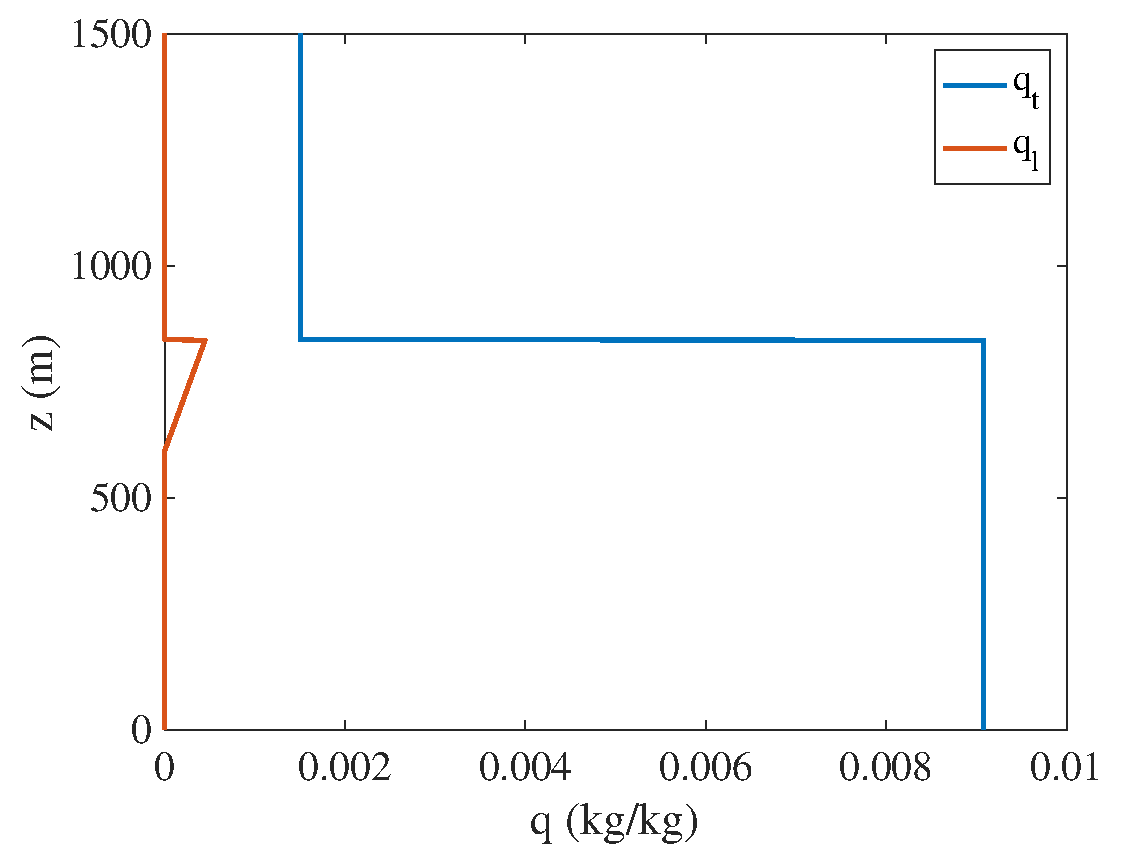
\includegraphics[width=0.49\textwidth]{./figures/dy_mixing_ratios.eps}
	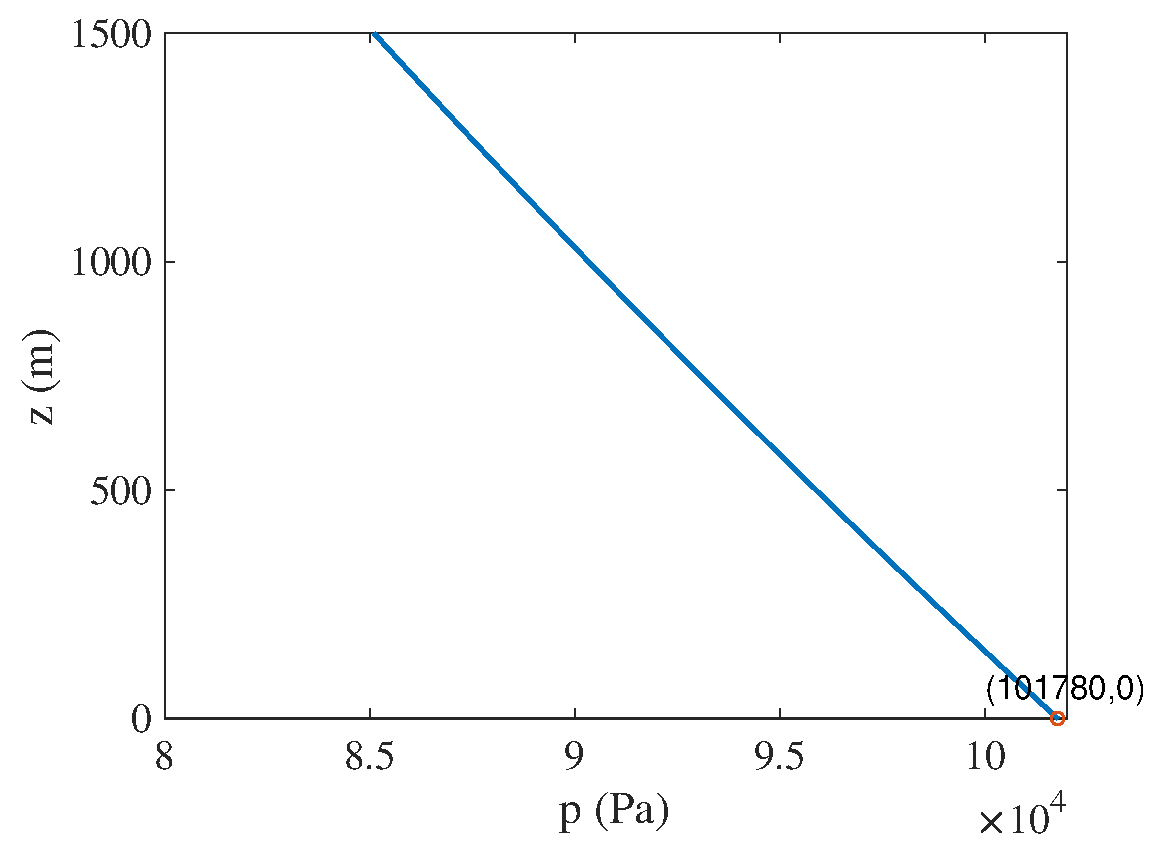
\includegraphics[width=0.49\textwidth]{./figures/dy_press.eps}
	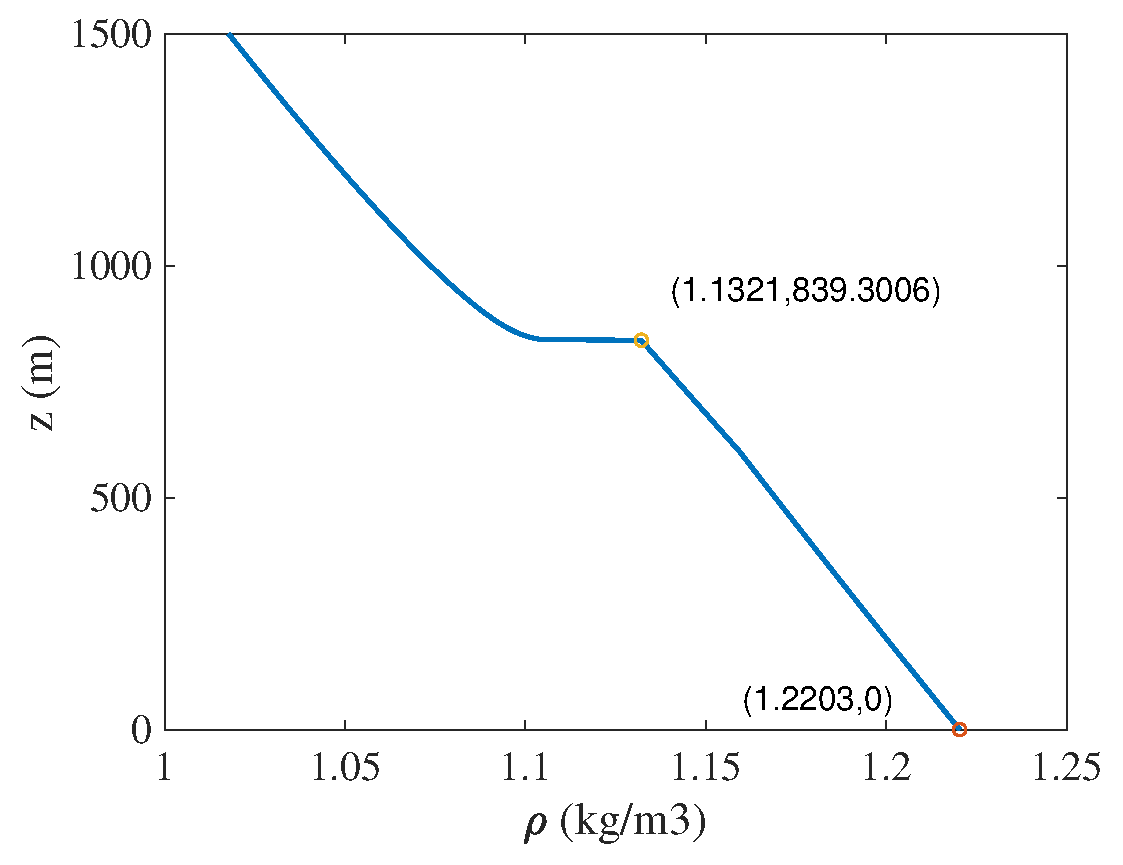
\includegraphics[width=0.49\textwidth]{./figures/dy_densi.eps}
	%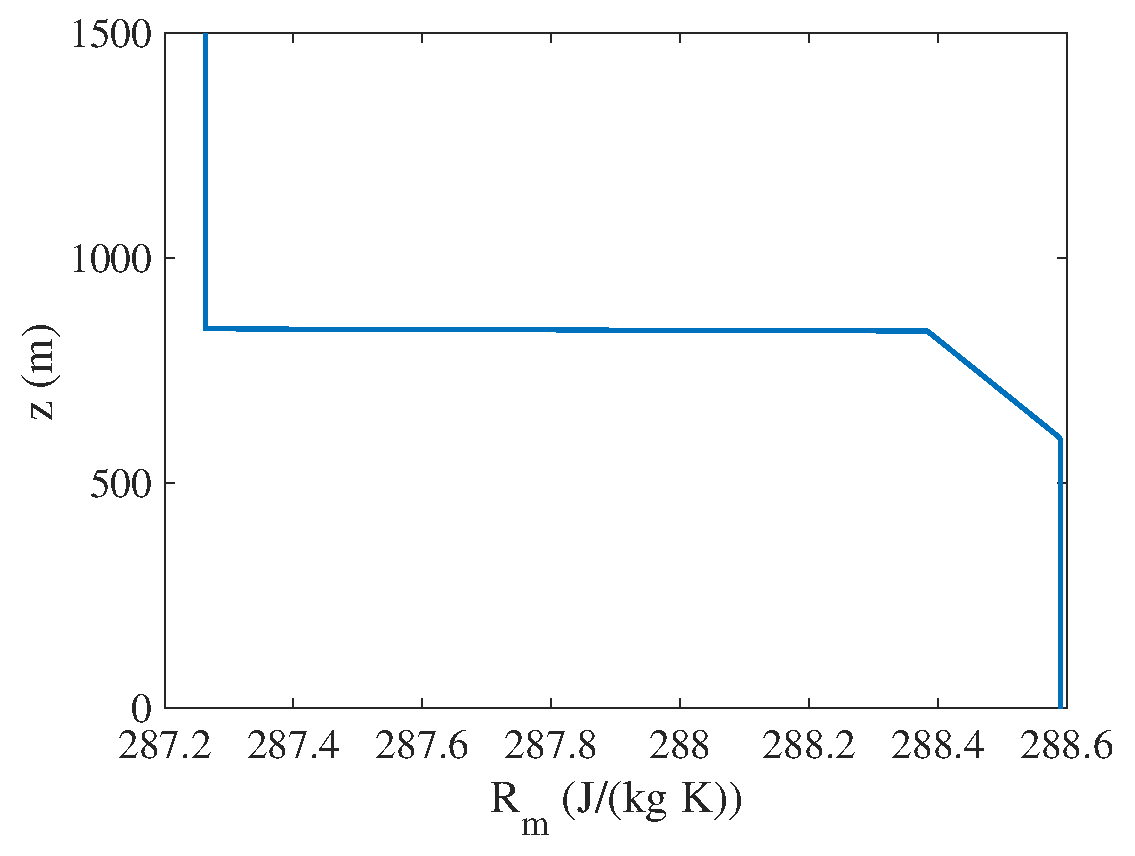
\includegraphics[width=0.49\textwidth]{./figures/dy_Rm.eps}
	%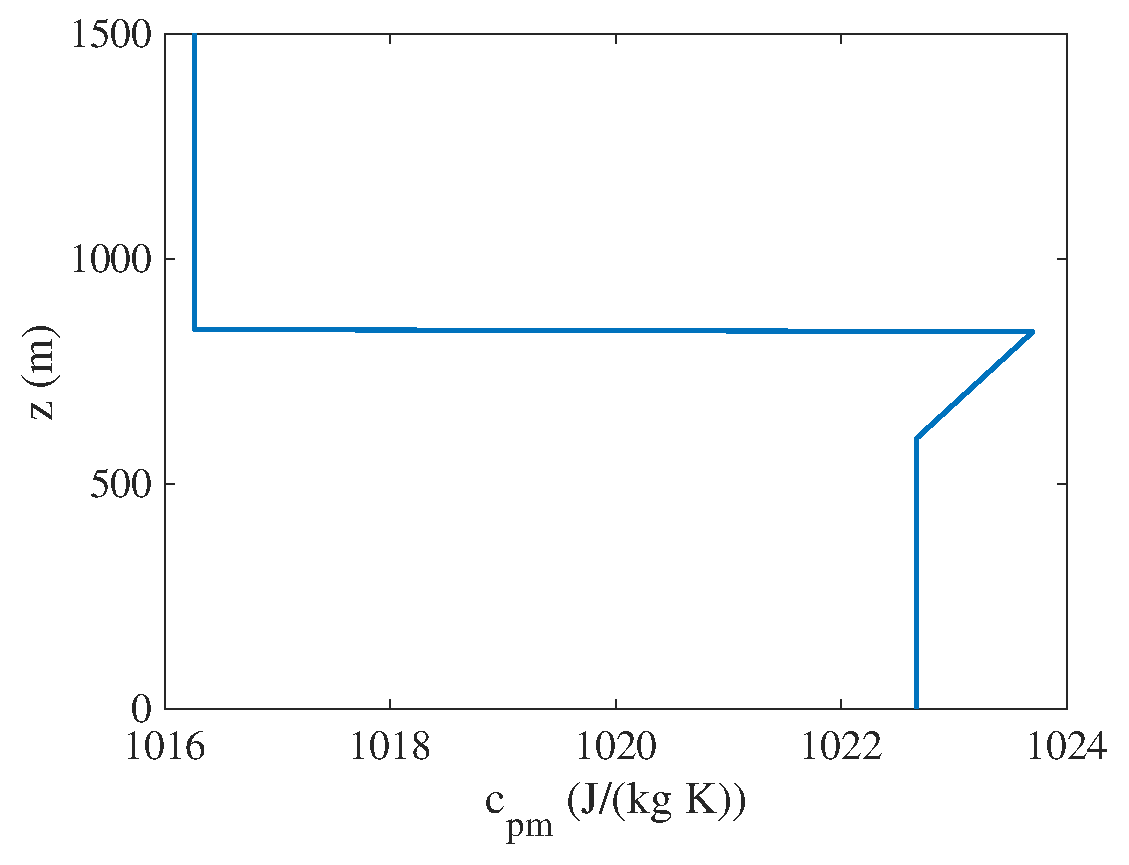
\includegraphics[width=0.49\textwidth]{./figures/dy_cpm.eps}
      \caption{Dycoms: initial states of $T, T_v, \theta, \theta_v, \theta_l, q_t, q_l, p, \rho$.}
\label{dycomsInitFig}
\end{figure}

\subsubsection{Boundary Conditions}

The bottom boundary conditions for DYCOMS are prescribed energy and water fluxes and a drag law for momentum, as described in section~\ref{s:bottom_bc}. The prescribed fluxes at the surfaces are
\begin{itemize} 
\item Sensible heat flux $\mathrm{SHF} = \vec{n} \cdot (\rho \vec{J}_{\mathrm{sfc}}) = 15\,\mathrm{W/m^2}$
\item Latent heat flux $\mathrm{LHF} = \vec{n} \cdot (\rho \vec{D}_{\mathrm{sfc}}) = 115\,\mathrm{W/m^2}$
\item Energy flux $\vec{n} \cdot \rho (\vec{J}_{\mathrm{sfc}} + \vec{D}_{\mathrm{sfc}}) = \mathrm{LHF + SHF} = 130\,\mathrm{W/m^2}$
\item Evaporation $E \approx \mathrm{LHF}/L_{v,0}$
\end{itemize}

\subsubsection{Sources}

\paragraph{Radiative cooling}
Radiative cooling is imposed through the simple model described by \cite{Stevens05a}. It specifies the vertical radiative energy flux $\vec{F}_R = F_R \vec{k}$ (part of the non-diffusive energy flux \eqref{eq:ndf_flux}) as
\begin{equation}
    \label{e:radiativeStevens05}
    F_{R}({\bf x}, t) = F_0{\rm e}^{-Q(z,\infty)} +
    F_1{\rm e}^{-Q(0, z)} +
    \rho_i c_{pd} D \alpha_z\frac{(z-z_i)^{4/3}}{4} + z_i(z - z_i)^{1/3}
\end{equation}
where 
\begin{equation}
    Q(a,b) = \kappa\int_{a}^{b}\rho\,q_l\,dz.
\end{equation}
The following parameters are used:
$F_0=70\,\mathrm{W\,m^{-2}}$, $F_1=22\,\mathrm{W\,m^{-2}}$, $\kappa=85\,\mathrm{m^2\,kg^{-1}}$, $\alpha_z=1\,\mathrm{m^{-4/3}}$. The parameter $D=3.75\times 10^{-6}\,\mathrm{s^{-1}}$ gives the large-scale divergence, which also enters the dynamical equations as an additional advection term.  

\paragraph{Large-scale subsidence}

A large-scale subsidence velocity $W=-Dz$ is imposed and is added to the internally generated vertical velocity $w$ in all governing equations. 

\subsubsection{SGS Fluxes}

The interaction of the resolved flow with SGS fluxes is crucial for a successful simulation of stratocumulus \citep{Pressel17a}. If there is too much spurious mixing across the sharp inversion interface, the clouds dissipate because too much dry air from above the clouds is mixed into the clouds. Hence, it is important to use SGS schemes that limit mixing near the stable inversion interface.

\section{3D Squall Line}
\label{sq3D}
The three-dimensional simulation of a squall line is defined in the domain 
$80\times 80\times20\,\mathrm{km}^3$. 
The initial background state is given by the sounding of \cite{gabersekGiraldoDoyle2012}.
To initiate the vertical transport of water vapor to a level of condensation (and hence trigger a cloud formation, the initial background is forced by a temperature anomaly $\theta'$ $3$ K warmer than the surrounding environment. 

A stretched grid along $z$ is used to make the resolution higher in the lower atmosphere where convection is triggered.
The domain is crossed by a horizontal wind along the x-direction with a $12\,\mathrm{m\,s^{-1}}$ shear at $z=2000\,\mathrm{m}$.
A no-slip condition is applied on the surface boundary while periodic boundaries are defined along $x$ and $y$. 
To damp the vertically propagating gravity ways triggered by the cloud formation, a Rayleigh absorbing layer is applied at the higher layers of the atmosphere.
The cloud first forms at approximately 500 s, and is fully develop after 4500 s. 
An instantaneous view of the precipitating squall line is shown in Figure \ref{fig:benchmarks/squall1}. 

\begin{figure}[htbp]
\includegraphics[width=1.2\textwidth]{figures/squall_working_warm_rain_frontal_view0028.png}
\caption{Front view of a fully developed squall line with precipitating rain. }
\label{fig:benchmarks/squall1}
\end{figure}


\section{External Soundings}
External soundings can be read into the code for initialization purposes. The sounding requires the format reported in Table \ref{tab:DeltaDefinitionsTable}.

\begin{table*}[t]
\centering
{\footnotesize
\caption[short]{Structure of sounding files for simulation initialization.}
\label{tab:DeltaDefinitionsTable}
\begin{tabular*}{\textwidth}{ @{\extracolsep{\fill}} llllll}
\hline
\hline
z (m) & $\theta_v$ (K) & $q_{tot}$ $\rm {kg/kg}$ & $u$ (m/s) & $v$ (m/s) & p (Pa)\\
0 & 300 & 14  & -2 & 0 & 100000\\
... & ... & ...  & ... & ... & ...\\
\hline

\hline
\hline
\end{tabular*}
}
\end{table*}

\bibliographystyle{agufull08}
\bibliography{Giraldo_refs,CLIMA-refs}

\end{document}
